% !TEX root = SLEBook.tex
\chapter{Rewriting}
Sometimes things look different but mean the same thing. For instance the mathematical expression $3+4$ evaluates to the same result as $4+3$. If we are only interested in the result of an expression, then we say they are {\em equal}, and we can write $3+4=4+3=7$.

If we are being very careful, then we would say that the expressions are equal {\em up to evaluation}. In some contexts, these expressions would not be thought of as equal. For instance the expression $3+4$ comprises three characters, and the expression $7$ only one, so if we are interested in how much storage we need in a computer to hold an expression, then $7$ is not equal to $3+4$.

An {\em equation} is two expressions separated by the {\em equality symbol} $=$. At a fundamental level, this tells is that the two expressions either side are interchangable because they evaluate to the same mathematical object, and that means that we can freely replace one by the other. It turns out that we can do a great deal of useful mathematics (and useful program translation) just by using equations.

For instance, imagine that we are given two complicated looking expressions and asked to decide if they are the same. Consider for instance the logical expressions

\[ a \land b... \]

Now we know a few facts about Boolean algebra. 

\section{Equality of programs}
In programming languages we are used to the idea of `equivalent' programs. For instance, this Java loop:
\begin{quote}
\begin{verbatim}
for (int i = 1; i < 10; i++) System.out.print(i + " ");
\end{verbatim}
\end{quote}
generates the same output as 
\begin{quote}
\begin{verbatim}
int i = 1; while (i<10) { System.out.println(i + " "); i++ }
\end{verbatim}
\end{quote}
If all we are interested in is output of a program, we might say that these two fragments are {\em equal} up to output, or just output-equal. More loosely, we often say that two programs are {\em semantically equivalent} if they produce the same effects. In this example, the iteration bounds are constant, and we could just have written
\begin{quote}
\begin{verbatim}
System.out.println("1 2 3 4 5 6 7 8 9 ")
\end{verbatim}
\end{quote}
These three fragments are semantically equivalent, but the third one will almost certainly run faster as it does not have the overhead of the loop counter and only makes one call to {\tt println()}. Our notion of semantically equivalent does {\em not} include performance, but only the values computed by a program.
\subsubsection*{Code improvement}
High quality translators for general purpose programming languages typically attempt to improve program fragments by surveying semantically equivalent alternatives, and selecting ones that are improvements with respect to some criteria. In the literature, these tools are usually called {\em optimising} compilers which is something of a misnomer since in general it is very hard to find a truly optimal implementation: perhaps they should be called code-improving compilers.
 
The conventional optimisation criteria are (i) execution speed, (ii) memory consumption and (iii) energy consumption. These three are not independent; for instance we can often speed things up by using more memory. Small battery operated systems will emphasise (iii) and (ii) over (i); high performance scientific computations such as weather prediction will emphasise (i).

In this book we are mostly interested in the meaning of programs up to, but not including, their performance, so we will have no more to say about code improvers and optimising compilers. However, there is a vast research literature describing often-ingenious techniques for improving program performance that you might wish to explore.

\section{Mathematical objects, their denotations and software implementations}
When thinking about programming languages, we need to carefully distinguish between (a) mathematical objects, (b) the textual forms (the denotations) that we use to name and manipulate those objects, and (c) the implementation of those objects inside a computer. 

\paragraph{Mathematical objects} When we are thinking mathematically, we are usually {\em imagining} abstract objects and operations regardless of whether we can make a concrete example. For instance we might decide to think about the set of all prime numbers, even though we have no easy way of deciding what the elements of that set are. We can give it a name (a denotation) and then go about investigating its properties: for instance Euclid proved that there must be infinitely many primes.

\paragraph{Denotations} When we are communicating about mathematics or programs we need conventions that enable us to write down what we mean. Consider the mathematical object that we get by adding unity to zero six times: we might denote that as $6$, $06$, {\em six} or {\em vi} (in Roman numerals). Which form we use is just a convention, and real programming languages usually support more than one convention: for instance Java allows us to write six as {\tt 6}, {\tt 06}, {\tt 0x06} or {\tt 0\_6} and these are all denotations for the same mathematical object.

\paragraph{Implementations} When we are programming a computer to perform addition we need some sort of {\em implementation} of an integer. Sadly, our implementations will never have the same properties as the mathematical integers, because our computers are finite. As a result in our programs there will always be some integer which, if we add one to it, will not generate the integer that mathematically we would expect. So, for instance, if we were using an eight-bit two's complement implementation of the integers, then $126 + 2$ would not generate 128 as that needs nine bits for its two's complement representation. On many systems, only the eight least significant bits would be retained, yielding {\tt -128}. Some systems have so-called {\em saturated} addition in which case the outcome would be 127 (the largest positive number in that representation). 

Note that even using arbitrary precision representations for integers such as Java's BigInteger we cannot faithfully represent mathematical integers as there will be an infinite set of integers that are too large to fit into our finite memory.

\section{String rewriting}

\section{Term rewriting}
\label{TermRewriting}
Programs often contain {\em expressions} such as \[17 / (4 + (x / 2)) \]They have a well-defined syntax: for instance $ 4 ) * (x + 2)$ is not a syntactically well formed expression because of the orphaned opening parenthesis. 

This particular way of writing expressions follows the style that we learn in school which makes use of {\em infix operators} like $+$ and $/$ to represent the operations of addition and division; they are called infix because are written in between the things they operate on. Expressions can nest and we understand that evaluation of an expression proceeds from the innermost bracket: to compute $17 / (4 + (x / 2))$ we first need to divide the value of $x$ by 2, then add 4, and then divide the result into 17.

The choice of infix notation is just that: an arbitrary choice, and we could have decided to use a different syntax to specify the same sequence of operations, such as \begin{quote}\begin{center}
\verb+divide(17, add(4, divide(x, 2)))+
\end{center}
\end{quote} We call this form a {\em prefix} syntax because each operation is written in front of the (parenthesized) list of arguments that it is to operate on.

Yet another form, often called {\em Reverse Polish Notation} enumerates the arguments and then specifies the operation:
\begin{quote}
\begin{center}
\verb+x,2,divide,4,add,17,divide+
\end{center}
\end{quote}

This format has the advantage that the operations are encountered in the order in which they are to be executed, and so no parentheses are required. That is a significant advantage, but many of us who grew up with infix notation find these sorts of expression hard to read.

All three of these forms are formally equivalent in that we can unambiguously convert between then without losing any information, and in fact it is easy to write a computer program to perform that conversion.

Although infix notation is familiar from everyday use it does not extend very comfortably to operations with more than two arguments. As a rare example: Java and C both provide the \verb+p ? et : ef+ notation for an expression in which predicate \verb+p+ is evaluated and then either expression \verb+et+ or expression \verb+ef+ is evaluated depending on whether the result of \verb+p+ was true or false.
 
In practice most programming languages provide infix notation for commonly understood operations such as addition, less than and logical-{\sc and}, but use prefix notation for other operations. Usually we can define procedures which are then called using a prefix notation. So, for instance, in Java we might write \begin{quote}\begin{center}\verb+System.out.println(Math.max(x,y))+\end{center}\end{quote}. 

If you are interested in the design of external language syntax then there are some alternatives to this approach that you might like to investigate. For instance Scheme and other LISP-like language use an exclusively prefix style; the printer control language PostScript uses Reverse Polish Notation; the Smalltalk language effectively uses an infix notation to activate all methods; the C++ language allows the dyadic operator symbols like \verb-+- to have their meanings extended to include new datatypes, and the Algol-68 language allowed completely new dyadic operator symbols to be defined. We shall return to these matters of syntactic style in Chapter~\ref{pragmatics}.
\section{Internal syntax style}
As language {\em implementors} and specifiers, we are mostly concerned with {\em internal} syntax\,---\,that is, how to represent programs compactly within the computer. We would like a general notation which is quite regular and thus does not require us to switch between different styles of writing what are essentially similar things. We should like to be able to easily transform programs so that if we chose, we could rewrite an expression such as $3+(5-(10/2))$ into $3+(5-5)$ or even $3$.

The {\em prefix} style is both familiar from mathematics and programming, and easy to manipulate inside the computer so we shall use that style almost exclusively to describe entire programs, and not just expressions. For instance the program
\begin{quote}
\begin{verbatim}
x = 2;
while (x < 5) { y = y * y; x++;}
\end{verbatim}
\end{quote}
might be written
\begin{quote}
\begin{verbatim}
sequence(assign(x,2), 
         while(greaterThan(x,5), 
               sequence(assign(y, mul(y, y)),
                        assign(x, add(x, 1)))))
\end{verbatim}
\end{quote}
Here, the concatenation of two statements X and Y in Java is represented by \verb+sequence(X, Y)+ and an assignment such as \verb+x = 2;+ by \verb+assign(x,2)+.

This notation has the great merit of uniformity: the wide variety of syntactic styles which are used in high level languages to improve program readability for humans is replaced by a single notation that requires us to firstly specify what we are going to do, say \verb+add+ and then give a comma-delimited parenthesised list of arguments that we are going to operate on.

The heavily nested parentheses can make this a rather hard-to-read notation although careful use of indentation is helpful. Sometimes, for small expressions at least, it can be helpful to use a tree diagram to see the expression. For instance $17 / (4 + (x / 2)) $, which we would write \verb+divide(17,add(4,divide(x,2)))+ can be drawn as 
\begin{center}
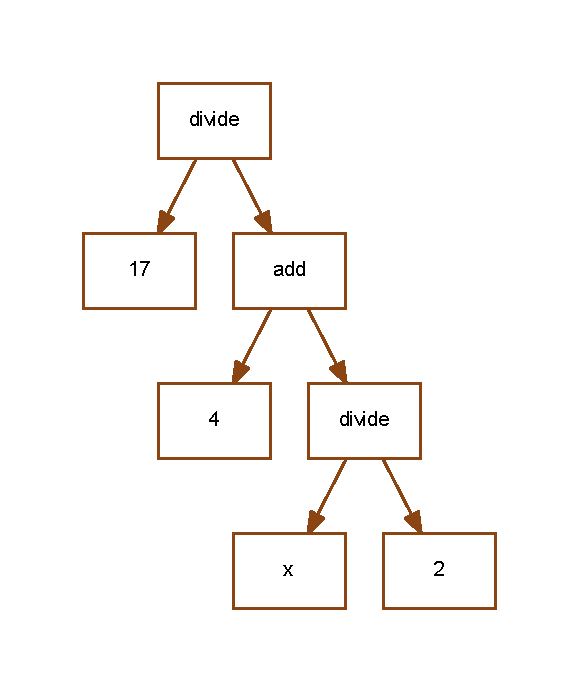
\includegraphics[scale=0.5]{pdf/semtree20.pdf}
\end{center}

\section{Terms}
We call the components of a prefix expression {\em terms}. Syntactically, we can define terms using an inductive (recursive) set of rules like this.
\begin{enumerate}
\item A symbol such \fbox{1}, \fbox{$\pi$} or \fbox{:=} is a term.
\item A symbol followed by a parenthesized comma-delimited list of terms is a term.
\end{enumerate}
Rule one defines terms made up of single symbols. Rule 2 is recursive,
and this allows us to construct terms of arbitrary depth by building
one upon another.

The {\em arity} of a term is the number of terms within its
parentheses. Terms from rule 1 have no parentheses: they are
arity-zero. Equivalently, the arity is the number of children a term
symbol has in its tree representation. Rule 1 terms have no children
and so are the leaves of a term tree.

Quite often, all instances of a symbol will have the same arity. For instance, addition is usually thought of as a binary (arity-two) operation, and an expression $3+4+5$ could be represented by the term \verb+add(add(3, 4),5)+. However, we could instead decide to have {\em variable} arity addition, in which case $4+4+5$ could be represented as \verb+add(3,4,5)+.


\subsection{Denoting term symbols}

We are very permissive about what constitutes a symbol. When we are thinking about theory, we allow the symbols to be any mathematical object. In this book, when we are thinking about computer based tools we shall allow a symbol to be {\em any} valid text string over the Unicode alphabet.

Now, great care is needed when reasoning about and writing down terms. Rule 2 above make comma and parentheses special: how would we go about writing a symbol that contained parentheses or command? We call these special characters {\em metacharacters} because they are used in the denotation of terms.
 
If we do want a parenthesis or a comma within a symbol, we usually write it with a
preceding back-slash (\verb+\( \) \,+ or sometimes back-quote
character. Of course, we have now added another meta-symbol, so if we
want a back-slash in a symbol name we have to write it as \verb+\\+.


\subsection{Typed terms}
Our definition of terms allows any term to be a subterm of any other term. Often we want to place constraints on our terms by limiting 
\section{Terms and their implementation in Java}
\label{TermsAndImplementation}
\newcommand{\str}{\mbox{\em Str}}
\newcommand{\nat}{\mbox{\em Nat}}
\newcommand{\obj}{\mbox{\em Obj}}

Assume that we have types \str (strings), \nat (natural numbers) and \obj (any data type). 

We can move from 
\begin{description}
\item [Pure text labels with embedded arity] $\str\ \mbox{label} \times \nat\ \mbox{arity} \times \mbox{term}^*$ 
\item [String map $\str\leftrightarrow\nat$]  $\nat\ \mbox{label} \times \nat\ \mbox{arity} \times \mbox{term}^*$
\item [Fixed arity map $\nat\leftrightarrow\nat$] $\nat\ \mbox{label} \times \nat\ \mbox{arity} \times \mbox{term}^* \lor \nat\ \mbox{label} \times \mbox{term}^*, \mbox{label} \in \mbox{arity map}$
\item [Types mapped to -1 in arity table, structure map $\nat\leftrightarrow\obj$] $\nat\ \mbox{label} \times \nat\ \mbox{data}$
\item [Small types bool, char, int and real mapped to negatives] $\nat\ \mbox{label} \times \mbox{data}$
\end{description}

Arrays should just be a vector of children


